\documentclass{cmn}

\begin{document}
  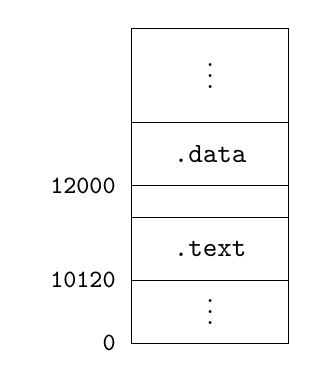
\begin{tikzpicture}
    \draw (0,0) -- ++(0,40mm) -- ++(20mm,0) -- ++(0,-40mm) -- cycle;
    \draw (0,8mm) -- ++(20mm,0);
    \draw (0,8mm+8mm) -- ++(20mm,0);
    \draw (0,20mm) -- ++(20mm,0);
    \draw (0,20mm+8mm) -- ++(20mm,0);

    \node[text width=10mm,align=right] at (-7mm,0mm) {\small\texttt{0}};
    \node[text width=10mm,align=right] at (-7mm,8mm) {\small\texttt{10120}};
    \node[text width=10mm,align=right] at (-7mm,20mm) {\small\texttt{12000}};

    \node at (10mm,12mm) {\texttt{.text}};
    \node at (10mm,24mm) {\texttt{.data}};

    \node at (10mm,5mm) {$\vdots$};
    \node at (10mm,35mm) {$\vdots$};
  \end{tikzpicture}
\end{document}
